\documentclass{beamer}

\usepackage{subfigure}
\usepackage{graphicx}
\usepackage{sidecap}
\usepackage{caption}
%\usepackage{subcaption}
\captionsetup{compatibility=false}
\usepackage{appendixnumberbeamer}
\usepackage{amsmath}
% --
\usepackage{multirow}
\usepackage{xcolor}
\usepackage{setspace}
\usepackage{hyperref}
\usepackage{anyfontsize}

\setbeamertemplate{footline}

\newenvironment{itemise} {\begin{itemize} \setlength{\itemsep}{0.2cm}} {\end{itemize}}
\usepackage[labelformat=empty]{caption}
\setbeamertemplate{sections/subsections in toc}[square]

%% COLORS
\definecolor{Gray}{gray}{0.9}
\definecolor{dblue}{rgb}{0.132,0.1,0.27}
\definecolor{mint}{cmyk}{1.0, 0.2, 0.6, 0.05}
\definecolor{ant}{cmyk}{0.5, 0.1, 0.0, 0.45}
\definecolor{lgray}{cmyk}{0.12, 0.0, 0.0, 0.17}
\definecolor{lred}{cmyk}{0.0, 0.9, 0.7, 0.0}


\usepackage{etoolbox}% http://ctan.org/pkg/etoolbox 
\usepackage{booktabs}

\newenvironment{literatur}{%
  \parskip2pt \parindent0pt \raggedright
  \def\lititem{\hangindent=0.5cm \hangafter1}}{%
  \par\ignorespaces}

\newcommand{\tb}[1]{{\color{blue}{\textbf{#1}}}}
\newcommand{\tm}[1]{{\color{mint}{\textbf{#1}}}}
\newcommand{\tr}[1]{{\color{red}{\textbf{#1}}}}
% Ilya: packages

\usepackage{tikz}
\usepackage{lmodern}
\usepackage{enumitem}

% Ilya: my commands

\newenvironment{mytemize}
{\vfill\itemize[nolistsep,itemsep=\fill,label=\color{blue}{$\triangleright$}]}
  {\enditemize}


\newenvironment{mynumerate}
{\vfill\enumerate[nolistsep,itemsep=\fill,label=\arabic*.]}
  {\endenumerate}

\newcommand{\hitem}[1]{
  {\color{blue}{$\triangleright$}} 
  {#1} 
  {\hfill}
}

\setlist[itemize]{label= \color{blue}{$\triangleright$}}
\setlist[enumerate]{label = \arabic*.}

\newcommand{\rarr}{$\Rightarrow$\ }



%\href{<Ziel>}{<Eingefasster Text>} 

%\logo{\includegraphics[height=0.7cm]{BdFlogo.eps}\hspace{300pt}\vspace{-5pt}}
%\logo{\includegraphics[height=0.8cm]{BdFlogo.eps}}
%\logo{\pgfputat{\pgfxy(-6.2,-0.5)}{\pgfbox[center,base]{\includegraphics[height=0.8cm]{BdFlogo.eps}}}}

%------------------------------------------------------------------------------------
% TITLE
%------------------------------------------------------------------------------------
\title[PSME]{Macroeconomics\\ Lecture 3 --- AD-AS, Time consistency of monetary policy} 
\author[I. Eryzhenskiy]{Ilya Eryzhenskiy}
\institute[BdF]{PSME Panth\'{e}on-Sorbonne Master in Economics}
\date[PSME macro]{Fall 2022}

%---BEGIN------------------------------------------------------------------------------
\begin{document}
%---BEGIN------------------------------------------------------------------------------
\begin{frame}
\maketitle
\end{frame}
%---FRAME------------------------------------------------------------------------------
\begin{frame}{Building theoretical Phillips curve: battle of markups}
\tb{Prices as mark-up on labour costs}\\
Firms with market power aim to set price as a markup over unit labor cost (or setting labor cost share):
\begin{align*}
P = (1+\theta) \frac{WL}{Y},
\end{align*}
where $\theta>0$ the markup.\\
\vfill
\tb{Wages as a mark-up on prices}\\
Workers (unions) bargain with firms for higher wages. \tr{Sticky wages}: negotiated wage fixed for some periods \rarr firms exposed to change of $\frac{W}{P}$ in the future under a fixed $W$ \rarr $P^e$ used in wage setting.  Bargaining determines firms' labor cost share under expected future prices $P^e$. In the negotiation, firms have reference price $\bar P$ and workers have reference (minimum) wage $\bar W$.
\begin{align*}
\frac{WL}{Y} = (1+\gamma)\bar{S}_L P^e,
\end{align*}
where $\bar{S}_L$ is reference labor cost share $\bar{S^L} = \frac{\bar W L}{\bar P Y}$ and $\gamma$ is the markup.
\end{frame}

\begin{frame}{From price to inflation: deriving AS and Phillips curve}
  Taking logs and total differential of the equation:
\begin{align*}
P &= (1+\theta)(1+\gamma)\bar{S}_L P^e \\
\ln P &= \theta+\gamma+\ln \bar{S}_L + \ln P^e \ (\text{as} \ \ln(1+x)\underset{x \to 0}{\to} x)\\
\text{total differential:} \frac{d P}{P} &= d \theta + d \gamma + \underbrace{\frac{d \bar S^L}{\bar S^L}}_{=0} + \frac{d P^e}{P^e} \\
\pi &= d \theta + d \gamma + \pi^e
\end{align*}
$\theta + \gamma$ \tb{procyclical} $\rightarrow d \theta + d \gamma = a \cdot Y^{gap}$ \rarr 
$$\pi = a \cdot Y_{gap}+ \pi^e$$ 
Finally, using \tb{Okun's law} to replace $Y^{gap}$ with $U^{gap}$:
$$\pi = -b \cdot U_{gap}+ \pi^e$$ 
\end{frame}

\begin{frame}{AS, Phillips Curve --- final form}
  Two elements are added to obtain full \tb{Phillips curve} and \tr{Aggregate Supply} relationships:
\begin{mynumerate}
\item Underlying rate of inflation $\tilde{\pi}$
\begin{mytemize}
\item generalization of expected inflation rate $\pi^e$ in wage setting 
\item wages sticky \rarr not only current expectations, but past expectations influence wage setting
\item explicit rules might exist for adjusting $W$ to $\pi$ \rarr past inflation rates enter $\tilde \pi$
\end{mytemize}
\item Supply shocks $s$
\begin{mytemize}
\item Shocks to non-wage marginal costs
\item Taken into account by firms when setting prices 
\end{mytemize}
\end{mynumerate}
\textbf{Results:}
\begin{align}
  \pi =& -b U_{gap} + \tilde{\pi} + s \tag{Phillips Curve}\\
\pi =& \quad a Y_{gap} + \tilde{\pi} + s \tag{AS}
\end{align}
\end{frame}

\begin{frame}{AS and Phillips curve: symmetry}
\begin{align}
  \pi =& -b U_{gap} + \tilde{\pi} + s \tag{Phillips Curve}\\
\pi =& \quad a Y_{gap} + \tilde{\pi} + s \tag{AS}
\end{align}
  \begin{center}
%{\small
%Figure. The output gap and unemployment in Germany, 1970-2016
%}
%\vspace{-2mm}
\begin{figure}[h!]
%	\subfigure{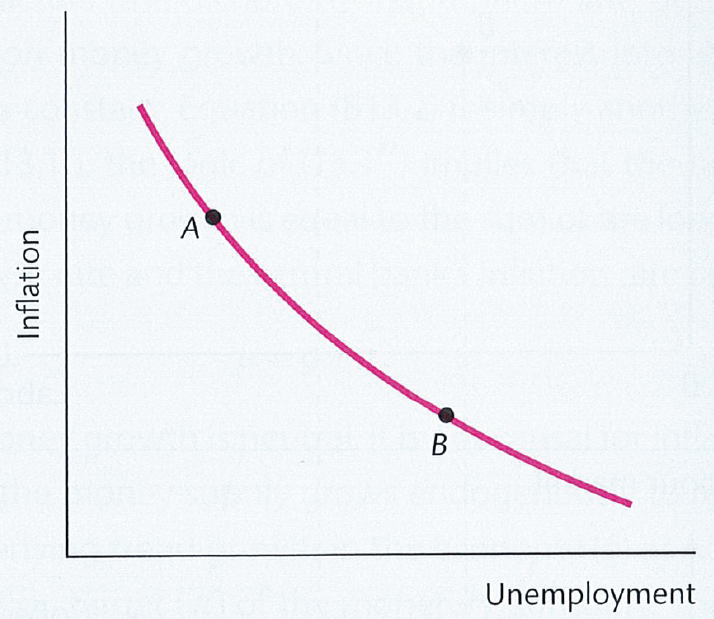
\includegraphics[trim=0 0 0 0,clip,width=0.45\textwidth]{FIGURES/8_PCtheory}
%	}      
	\subfigure{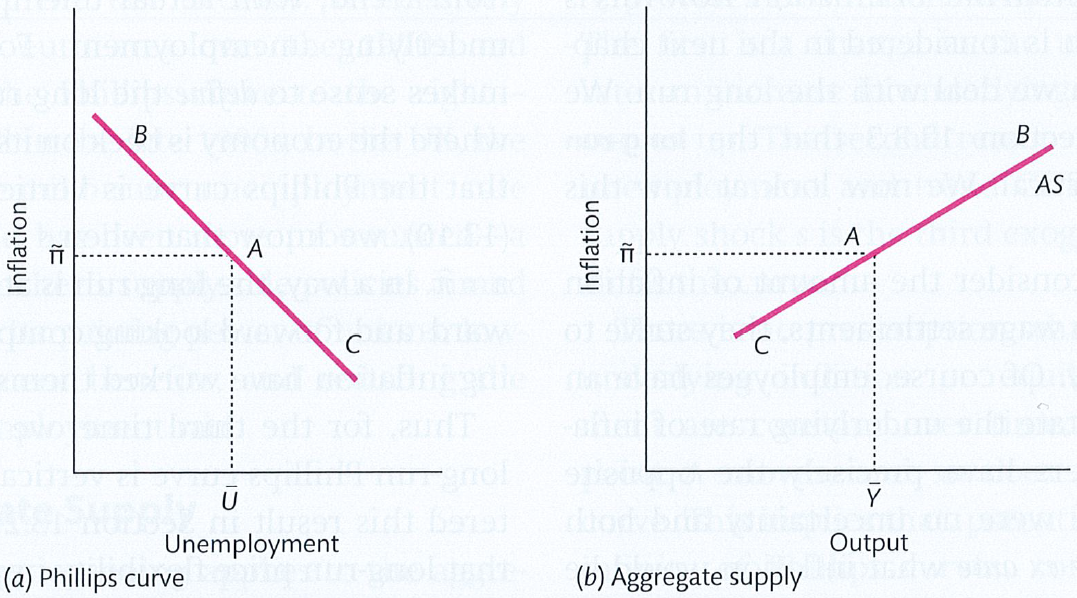
\includegraphics[trim=0 00 0 00,clip,width=0.9\textwidth]{FIGURES/8_NewPC}
	} 	
	%[trim=left bottom right top
\end{figure}
%\vspace{-2mm}
\begin{minipage}{0.90\columnwidth}
\tiny	
\textbf{Note.} The new Phillips curve. \textbf{Source.} Burda and Wyplosz (2017), Figure 13.12.\\
\end{minipage}
\end{center}
\end{frame}
%---FRAME------------------------------------------------------------------------------
\begin{frame}{Non-labor costs and supply shocks}

  Firms have small supply shocks all the time, but which ones are macroeconomic? \\
  \vfill
  \tr{Energy prices}, especially fossil fuels, have a big role:
\begin{itemize}
\item First oil shocks: 1973/74, 1979/81
\item Second sequence of shocks: 1999/2001, 2005/12
\item Favourable oil shocks: 1986 and 2015
\item Current: war \& sanctions \rarr Russian oil shut off: 2022
\end{itemize}

\begin{center}
  \begin{figure}[h]
	\centering
	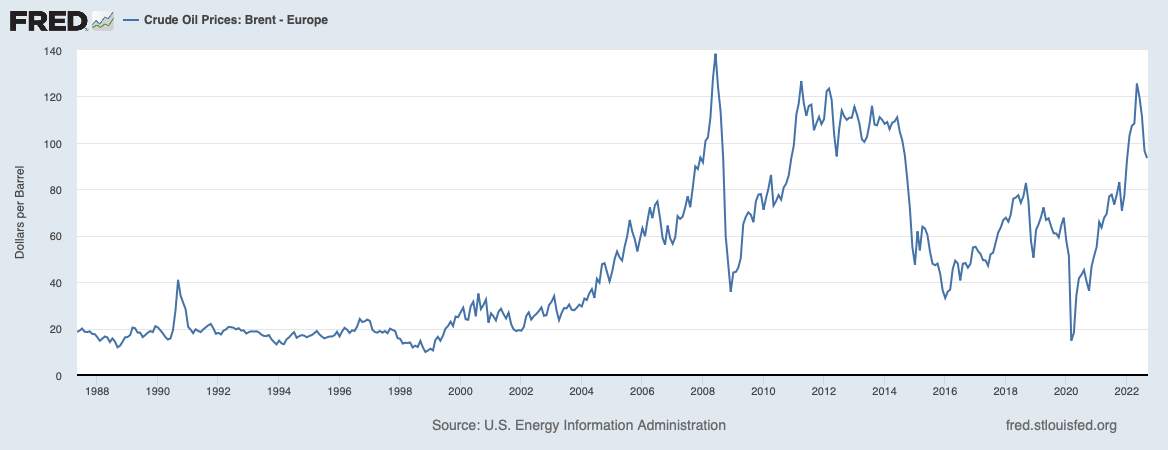
\includegraphics[width = \textwidth]{FIGURES/brent_190922.png}
  \end{figure}
\begin{minipage}{0.5\columnwidth}
\tiny	
Brent Europe crude oil price. \textbf{Source.} St. Louis Fed. \\
\end{minipage}
\end{center}
%\begin{center}
%{\small
%Figure. The output gap and unemployment in Germany, 1970-2016
%}/
%\vspace{-2mm}
\end{frame}
%---FRAME------------------------------------------------------------------------------
\begin{frame}{Underlying inflation, long-run Phillips curve}

\begin{mytemize}
\item \tb{Rational expectations} 
\begin{itemize}
\item Forecast errors occur, but must average to zero over longer horizons
\item Differences in $\pi$ and $\tilde{\pi}$ must be temporary
\item Long-run link equivalence of actual and underlying inflation:\\
if $s=0$ and $U=\bar{U}$, then $\pi=\tilde{\pi}$
\end{itemize}
\item Implies a \tr{vertical Phillips Curve in the long run}
\item The level of \tr{long run inflation}? 
  \begin{mytemize}
  \item[$\rightarrow$] $\bar \pi$, \tr{inflation target of the central bank}.
  \end{mytemize}
\end{mytemize}
\end{frame}
%---FRAME------------------------------------------------------------------------------
\begin{frame}{Long-run Aggregate Supply (LAS)} 

\begin{mytemize}
  \item Recall that \tb{trend output} $\bar Y$ determined by technology, demographics
	\begin{mytemize}
	\item No relation of $\bar Y$ level to $\pi$ \rarr \tr{vertical LAS}
	\end{mytemize}
\item Another way to obtain --- long-run Phillips curve \& Okun's law 
%\item It shifts with changes in exogenous variables ($\tilde{\pi},\bar{Y},s$)
  \end{mytemize}
 \textbf{Implications:}
\begin{mytemize}
\item \tm{Short run}: Actual inflation deviates from underlying inflation $\tilde{\pi}$ in tandem with the business cycle
\item \tm{Long-run}: output returns to its growth path, independent of price level. 
  \begin{mytemize}
  Horizontal movement due to trend output $\bar{Y}$ growing at rate $g$
  \end{mytemize}
\end{mytemize}

\end{frame}
%---FRAME------------------------------------------------------------------------------
\begin{frame}{Shifts in Phillips curve and AS --- unstable relationships}

\begin{mytemize}
\item $\tilde{\pi},\bar{U},\bar{Y},s$ are taken as exogenous and can shift the curves
\item[$\rightarrow$] a set of Phillips curves, not a stable negative relationship
\item A. W. Phillips was \textbf{lucky} to find one stable curve
\item At least to strong reasons for shifts since 1970s:
\begin{mytemize}
\item Supply shocks (oil prices)
\item Shifts in the equilibrium unemployment rate
\end{mytemize}
\end{mytemize}
\begin{center}
{\tiny
Figure. United Kingdom, 1970-2015
}
\vspace{-3mm}
\begin{figure}[h!]
%	\subfigure{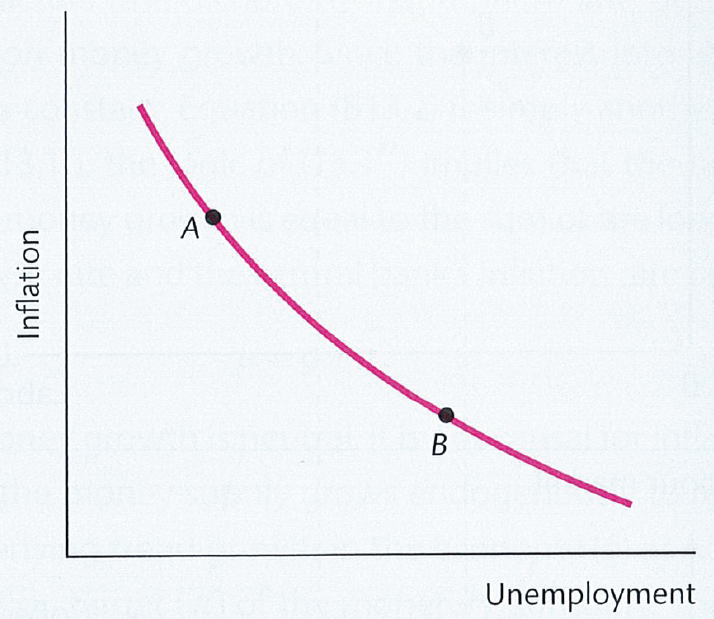
\includegraphics[trim=0 0 0 0,clip,width=0.45\textwidth]{FIGURES/8_PCtheory}
%	}      
	\subfigure{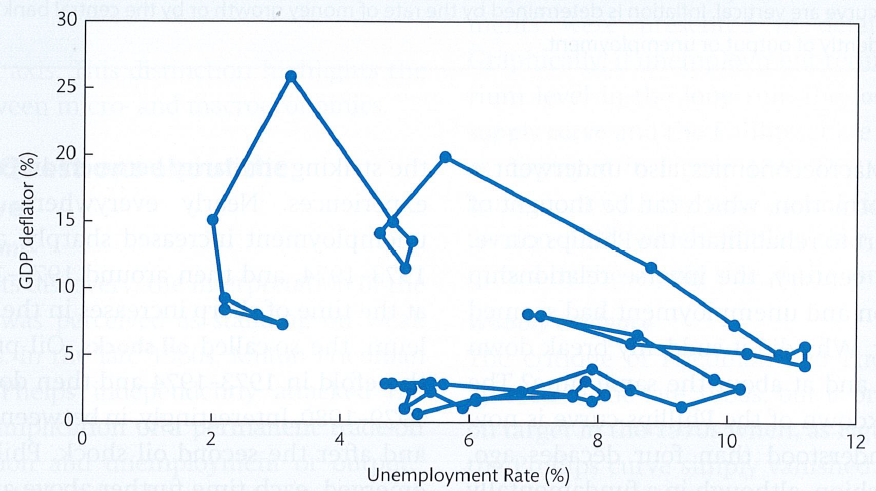
\includegraphics[trim=0 00 0 00,clip,width=0.55\textwidth]{FIGURES/8_PCdataUKpost70}
	} 	
	%[trim=left bottom right top
\end{figure}
%\vspace{-2mm}
\begin{minipage}{0.50\columnwidth}
\tiny	
\textbf{Source.} Burda and Wyplosz (2017), Figure 13.10.\\
\end{minipage}
\end{center}

\end{frame}
%---FRAME------------------------------------------------------------------------------
%\begin{frame}{Changes in equilibrium unemployment over time}
%
%\begin{itemize}
%\small
%\item Upward trend: 1970-2000/10
%\item Downward trend: 2000/10-2015
%\end{itemize}
%\begin{center}
%%{\small
%%Figure. The output gap and unemployment in Germany, 1970-2016
%%}
%%\vspace{-2mm}
%\begin{figure}[h!]
%%	\subfigure{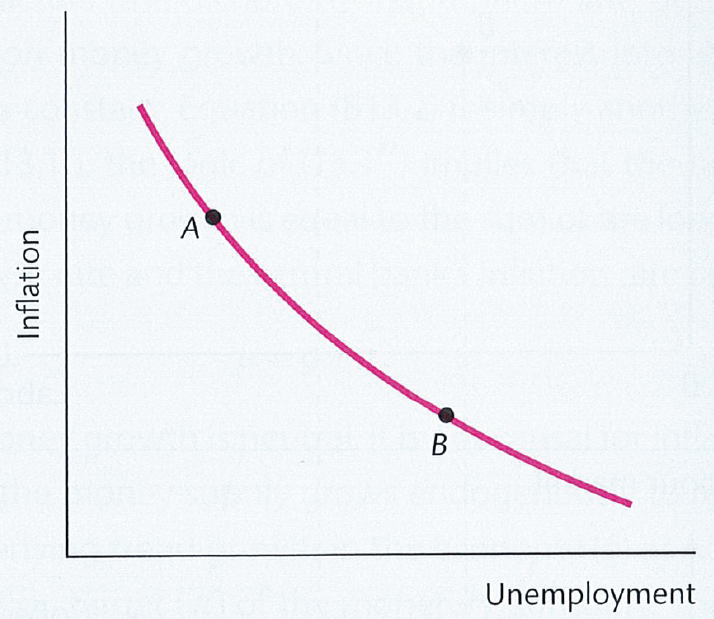
\includegraphics[trim=0 0 0 0,clip,width=0.45\textwidth]{FIGURES/8_PCtheory}
%%	}      
%	\subfigure{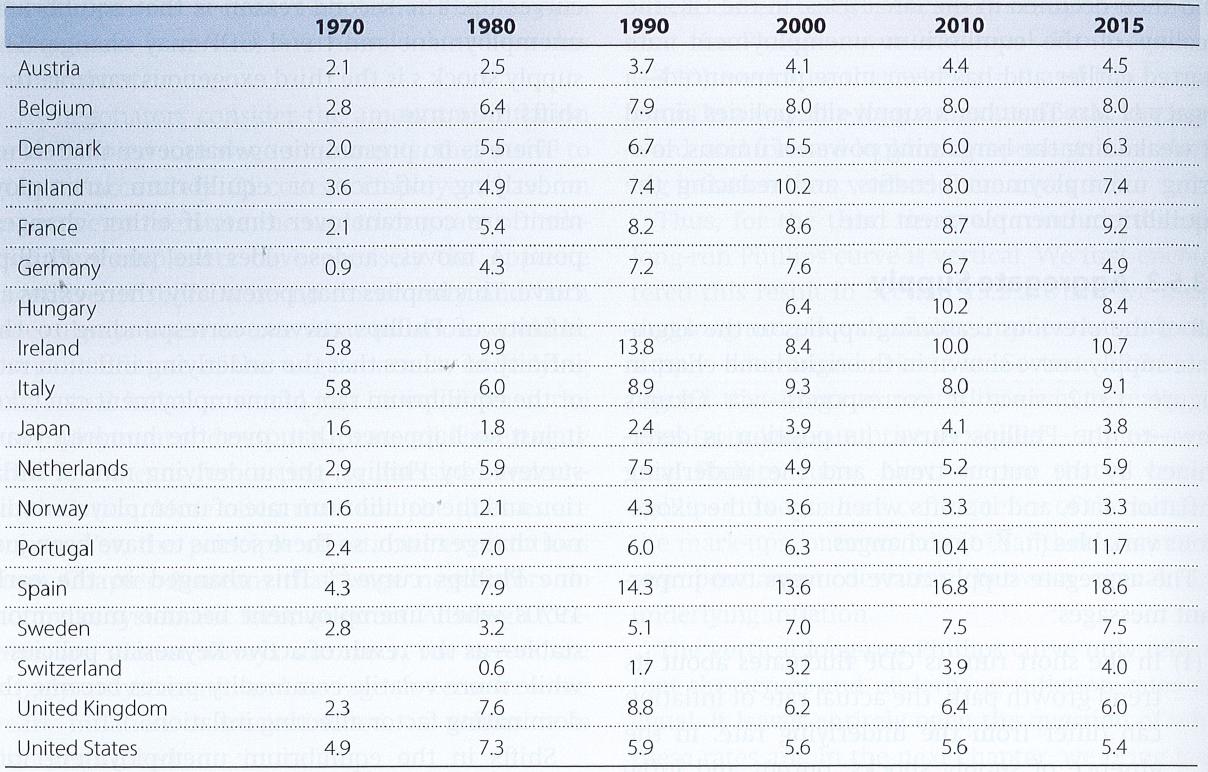
\includegraphics[trim=0 00 0 00,clip,width=0.85\textwidth]{FIGURES/8_TableNAIRU}
%	} 	
%	%[trim=left bottom right top
%\end{figure}
%%\vspace{-2mm}
%\begin{minipage}{0.90\columnwidth}
%\tiny	
%\textbf{Note.} NAIRU = nonaccelerating inflation rate of unemployment (What unemployment rate would keep the Phillips curve unchanged if $\tilde{\pi}=\pi$ and $s=0?$). \textbf{Source.} Burda and Wyplosz (2017), Table 13.2.\\
%\end{minipage}
%\end{center}
%
%\end{frame}
%---FRAME------------------------------------------------------------------------------
\begin{frame}{Phillips curve and AS: summary} 
\begin{mytemize}
\item Instead of a simple $U, \pi$ relationship found originally, theoretical Phillips curve is more flexible:
\begin{mynumerate}
\item Short-run Phillips curve depends on expectations and supply shocks
\item Long-run Phillips curve is vertical --- no inflation-unemployment link
\end{mynumerate}
\item Via \tb{Okun's law}, short-run and long-run \tb{AS} are obtained
\end{mytemize}

\begin{center}
\begin{figure}[h!]
%	\subfigure{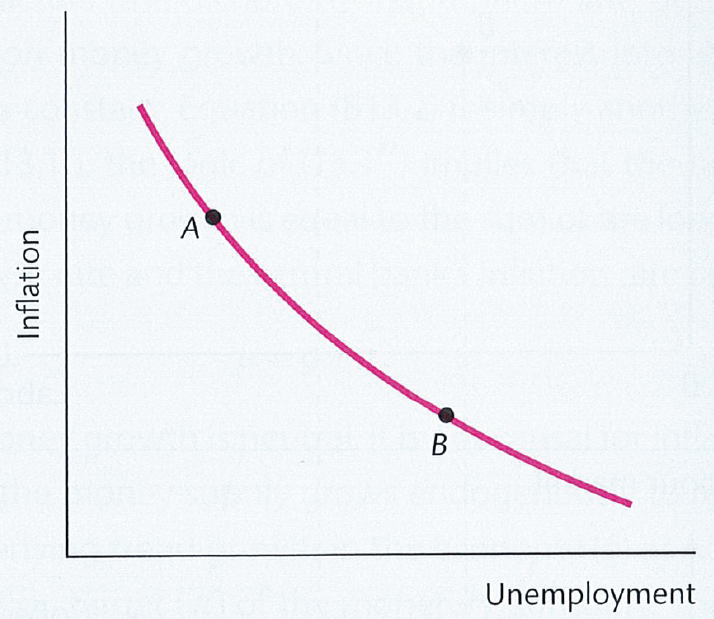
\includegraphics[trim=0 0 0 0,clip,width=0.45\textwidth]{FIGURES/8_PCtheory}
%	}      
	\subfigure{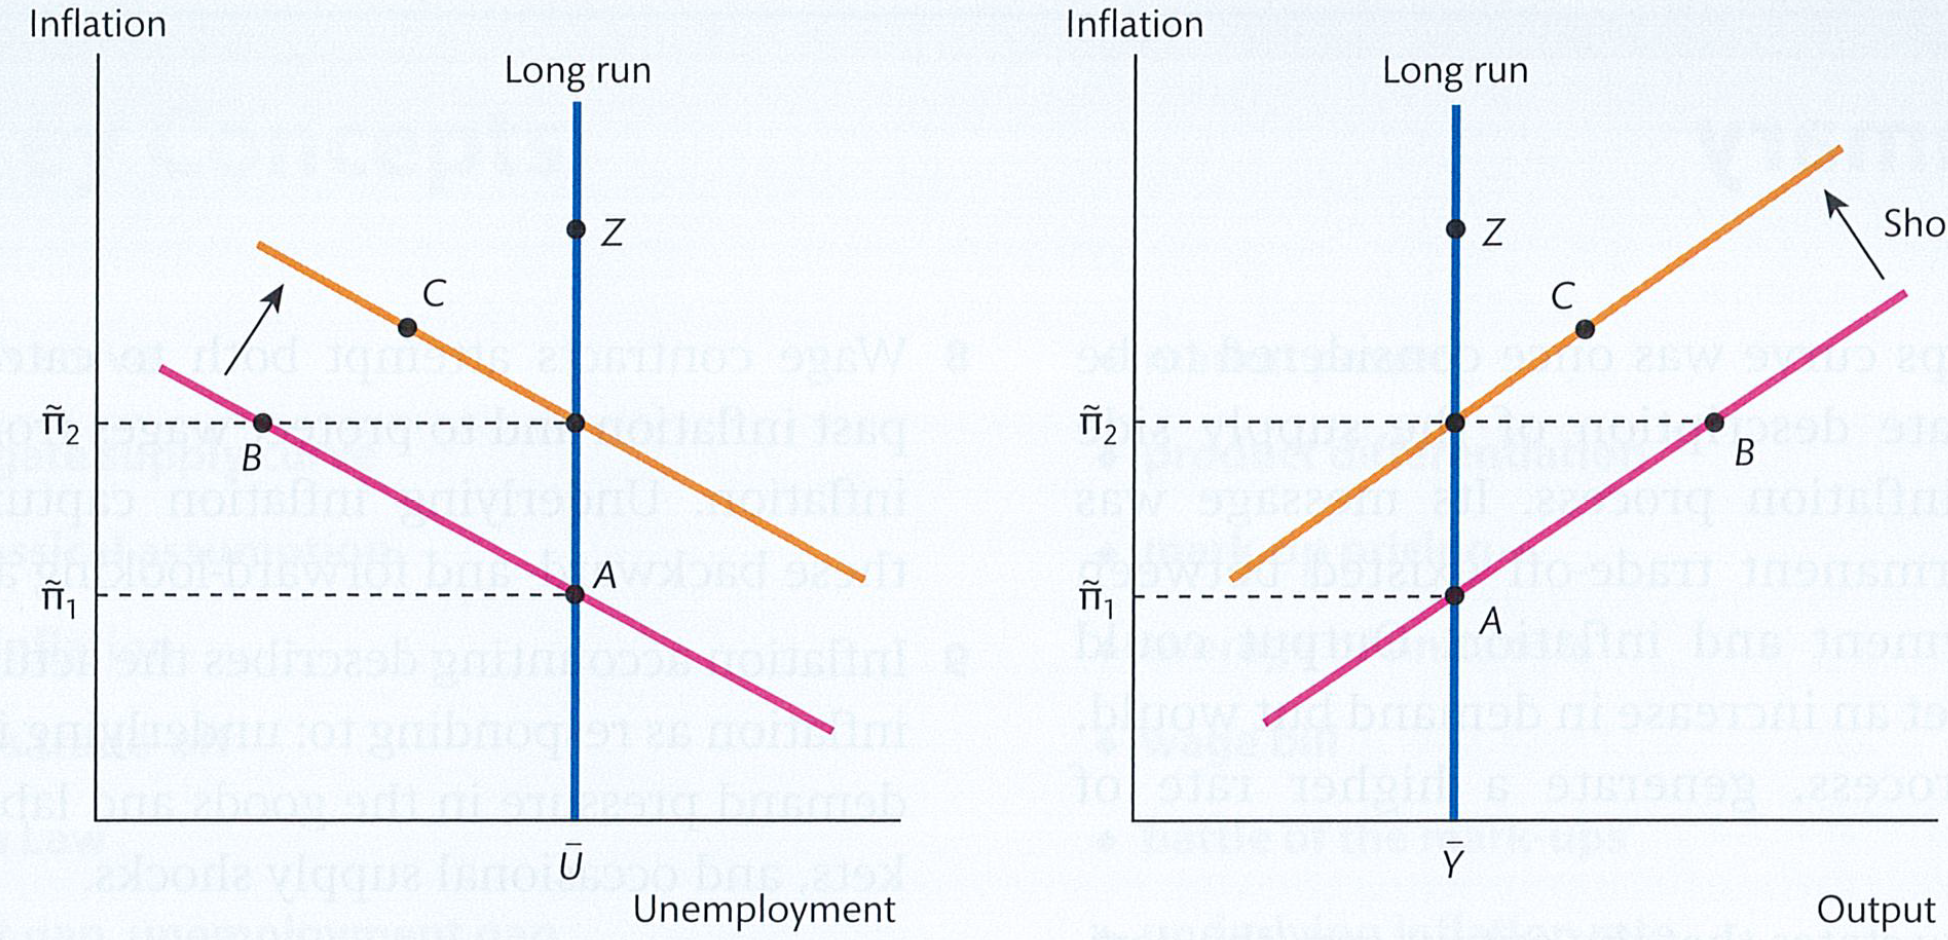
\includegraphics[trim=0 0 0 0,clip,width=0.9\textwidth]{FIGURES/8_TransitionShortLong}
	} 	
	%[trim=left bottom right top
\end{figure}
\vspace{-2mm} \begin{minipage}{0.50\columnwidth}
\tiny	
\textbf{Source.} Burda and Wyplosz (2017), Figure 13.13.\\
\end{minipage}
\end{center}
\end{frame}
%---FRAME------------------------------------------------------------------------------
\section{AS-AD model}
\begin{frame}{AD-AS model}
  \begin{mytemize}
  \item Medium-term movements of output and inflation shaped by both supply and demand
  \item \tb{AS} is obtained above
  \item \tr{AD} follows immediately from the IS-TR model with full version of TR:
  $$i = \bar i + \textcolor{red}{\alpha (\pi - \bar \pi)} + \beta \left(\frac{Y- \bar Y}{\bar Y}\right)$$
  \end{mytemize}
\end{frame}


\begin{frame}{Long-run AD (LAD)}
  \begin{mytemize}
	\item In the long run, central bank assumed to set interest such that $\pi = \bar \pi$ for whatever $Y$ (which is $\bar Y$ in equilibrium) 
	\begin{mytemize}
	\item horizontal \tb{LAD}
	\item will become more relevant in open economy analysis
	\end{mytemize}
  \end{mytemize}
\begin{center}
%{\footnotesize
%Figure. Exchange rate of Danish krona vis-a-vis (a) EUR and (b) USD  \\
%}
%\vspace{-2mm}
\begin{figure}[h!]
%\caption{Figure. Net}
	\subfigure{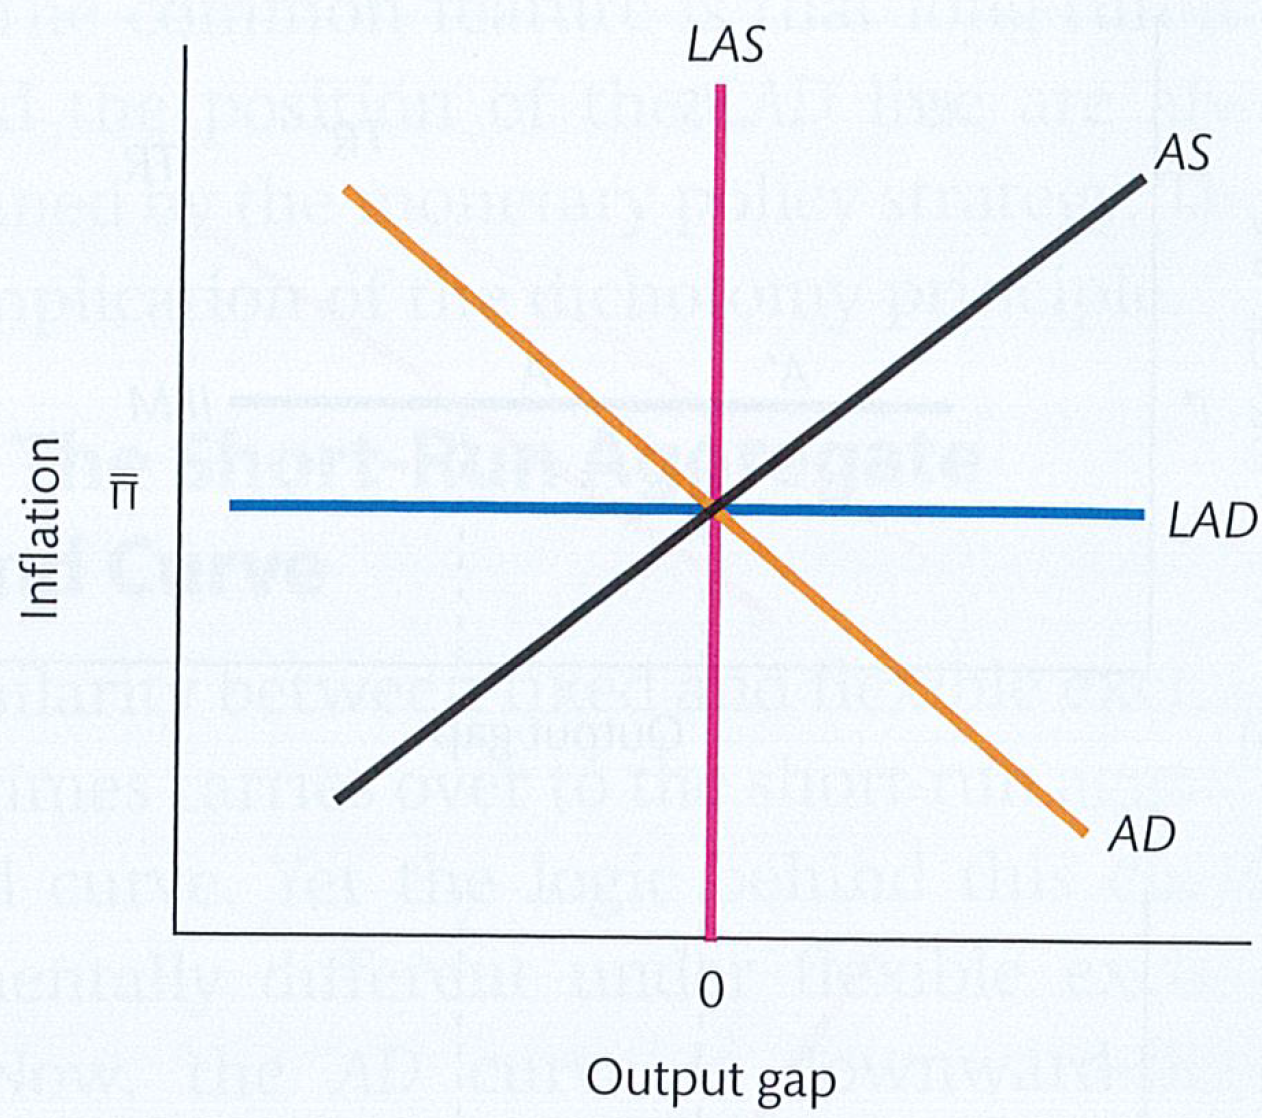
\includegraphics[trim=0 0 0 0,clip,width=0.45\textwidth]{FIGURES/9_ASAD_Flexible}
	}      
	%} 		
%	\label{fig:GPD} 
	%[trim=left bottom right top
\end{figure}
%\vspace{-2mm}
\begin{minipage}{0.5\columnwidth}
\tiny	
%\textbf{Note.} Inflation in Denmark and the euro area (1992-2016).  
\textbf{Source.} Burda \& Wyplosz (2017), Figure 14.12.\\
\end{minipage}
\end{center}
\end{frame}
%---FRAME------------------------------------------------------------------------------
%---FRAME------------------------------------------------------------------------------
\begin{frame}{Short run AD}

\begin{columns}
\column{0.5\linewidth}
Assume an increase in $\pi$:
\begin{itemize}
  \item TR: Central bank raises interest rate 
\item Investment decreases, $IS$ shifts to the left
\item Equilibrium $Y$ lower for higher $\pi$: downward sloping short run \tb{AD}
\end{itemize}
\tb{Shifts in AD}
\begin{itemize}
  \item IS: any shift in desired demand
  \item \emph{TR}: $\bar Y, \bar{\pi}$
%\item \emph{IFM}: $\Delta i^* \neq 0$
\end{itemize}
% COLUMN(2)
\column{0.45\linewidth}
\vspace{7cm}
 AD \& IS-TR:

\end{columns} 	 

\end{frame}
\begin{frame}{Policy example: monetary policy}
  \vspace{-3cm}
 \small \tb{Higher inflation target}, $\bar{\pi}'> \bar{\pi}$
 \vfill
\end{frame}

\begin{frame}{Policy example: government spending}
  \vspace{-3cm}
  \small \tb{Positive fiscal policy shock}, $\bar{G}'> \bar{G}$, either permanent or temporary
 \vfill
\end{frame}

\begin{frame}{AS once again}
  A short-medium run AS relationship $\pi = a (y - \bar y) + \tilde \pi + s$ arises in \textbf{many} models, under different assumptions.  
  \begin{mytemize}
  \item We have focused on price-wage-expected price link through \tb{markup} price and wage setting, with \tb{pro-cyclical} markups
	\begin{mytemize}
	\item Story went like output/unemployment gap $\rightarrow$ inflation
	\end{mytemize}
  \end{mytemize}
  \vfill
  AS can also go in inflation $\rightarrow$ output direction:
	\begin{mynumerate}
	\item Sticky wages \rarr when $\pi \uparrow$, $\frac{W}{P} \downarrow$, so firms more profitable and $(y - \bar y) \uparrow$
	\item Multiple goods, incomplete information in firms \rarr when $\pi \uparrow$, firms cannot distinguish \tr{inflation} (e.g. due to monetary policy) from \tr{relative price movements} (e.g. due to changes in preferences) \rarr each firm produces more, since demand might be rising for their particular product only (Lucas, 1972)
	\end{mynumerate}
	\vfill
	Can rewrite AS to highlight inflation $\rightarrow$ output: \\
	$y = \bar y + a' (\pi - \tilde \pi) + e, \quad \text{where} \quad a' = 1/a, e = -1/a \cdot s $

\end{frame}

\section{Monetary policy and time consistency}
%\section{Outline}
\begin{frame}
\frametitle{Outline}
\tableofcontents[currentsection]
\end{frame}

%---FRAME------------------------------------------------------------------------------
%---FRAME------------------------------------------------------------------------------

\begin{frame}{Discretionary policy and time-inconsistency}

\begin{itemize}
  \item Central banks often independent from political influence. \tr{Why?}
\item Negative correlation between measures of central bank independence and inflation: %(Cukierman 1992)
\item[$\rightarrow$] An independent central bank with a focus on price stability is a solution to \tb{time consistency} problems in monetary policy
\end{itemize}

\begin{center}
%{\footnotesize
%\textbf{Figure.} Target corridors and realized inflation rates. \\
%}

%\vspace{-2mm}
\begin{figure}[h!]
%\caption{Figure. Capital share US, 1946-2018
	%\subfigure{\includegraphics<1>[trim=80 60 100 70,clip,width=0.75\textwidth]{FIGURES/3_Autarky}
	%}
	\subfigure{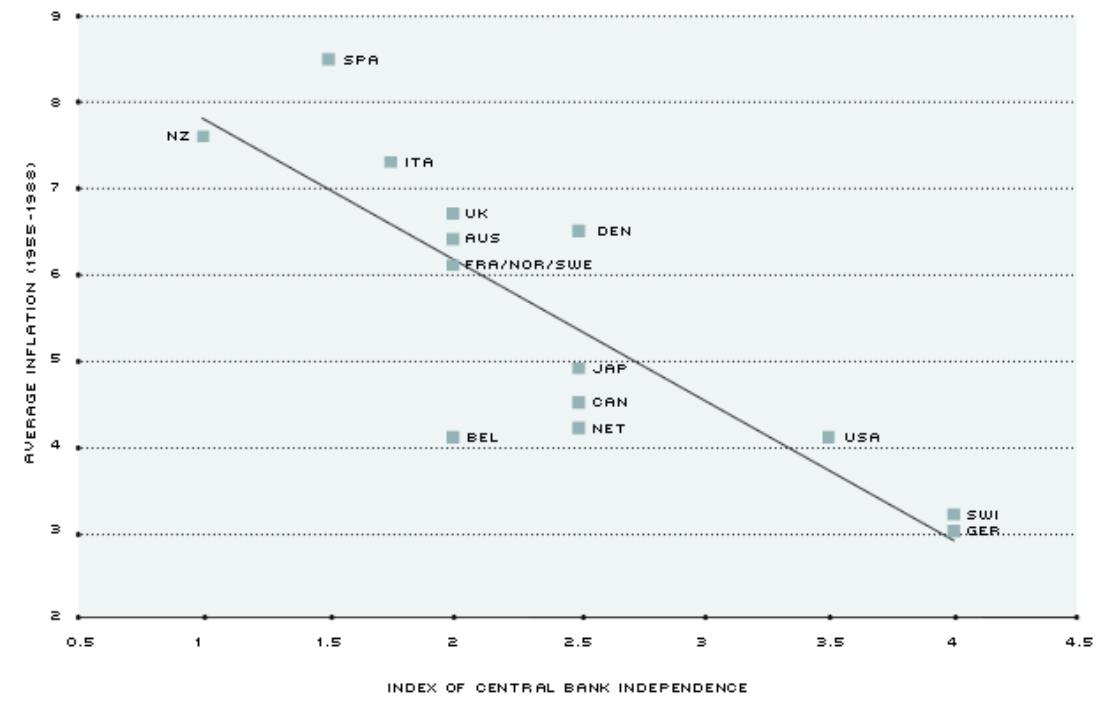
\includegraphics[trim=0 0 0 0,clip,width=0.7\textwidth]{FIGURES/5_CBI}
	}      %\\
	%\subfigure{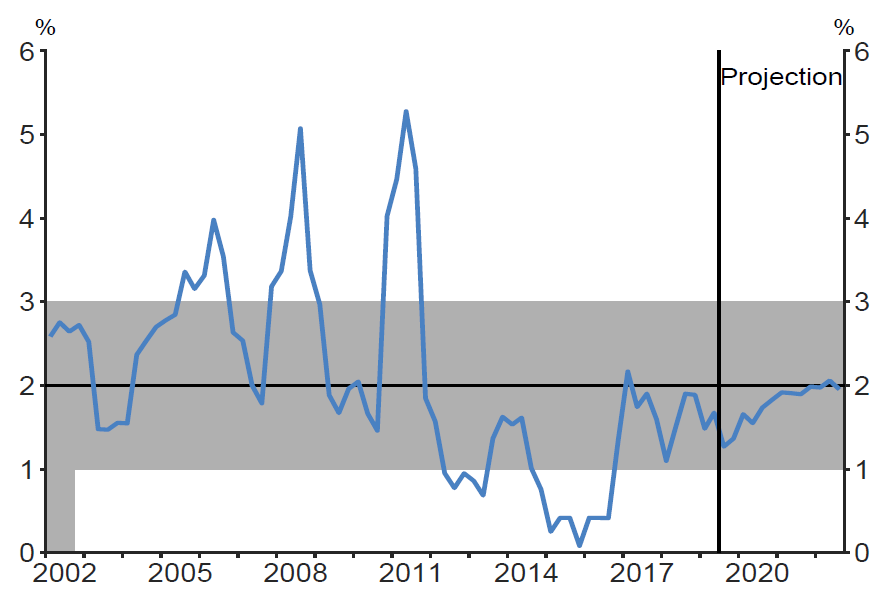
\includegraphics[trim=0 0 0 0,clip,width=0.35\textwidth]{FIGURES/5_NZforecast}
	%} 
	
%	\label{fig:GPD} 
	%[trim=left bottom right top
\end{figure}
%\vspace{-2mm}

\begin{minipage}{0.92\columnwidth}
\tiny	
%\textbf{Note.} Signatures on US dollar banknote by Rosa Gumataotao Rios and Timothy F. Geithner
\textbf{Sources.} Federal Reserve Bank of St. Louis Annual Report 2009, Figure 1. \\
\end{minipage}
\end{center}
\end{frame}
%---FRAME------------------------------------------------------------------------------
\begin{frame}{Time consistency of monetary policy: framework}

\begin{mytemize}
\item Central bank (CB) cares for both GDP and inflation
  \begin{mytemize}
  \item influences inflation, but also indirectly GDP though \tb{AS}
  \end{mytemize}
\item private agents guess CB's actions and form \tr{inflation expectations}
\item monetary policy can either be \tb{discretionary} (CB free to change policy) or \tb{rule-based}
\end{mytemize}

\textbf{Main results}
\begin{mynumerate}
\item CB uses inflation to boost GDP \rarr cannot credibly promise low inflation: \tb{time inconsistency} problem
\item Discretionary policy \rarr higher inflation, which is anticipated \rarr no output gain
\item Rules-based policy \rarr can promise lower inflation, but still respond to supply shocks
\end{mynumerate}

\end{frame}

\begin{frame}{The model (Barro, Gordon, 1983)}

\tb{Central bank}: maximize utility/minimize cost:
\begin{align*}
\max_{\pi} U(y-\bar y, \pi)
\end{align*}
\tb{AS} relationship of inflation and output:
	$$y = \bar y + a (\pi - \pi^e) + e$$
	where $e$ supply shock; expected inflation $\pi^e$ used as \textbf{underlying inflation}
\vfill
\tb{Private agents}: know CB's preferences, have \textbf{rational} inflation expectations $\pi^e$

\end{frame}

\begin{frame}{Sequence of events}

  Timeline very important for understanding the model:
\begin{mynumerate}
\item Private sector guesses monetary policy based on CB preferences \rarr inflation expectations $\pi^e$
\item Supply shock $e$ realizes
\item Monetary policy made: $\pi$ chosen by CB
\end{mynumerate}
\vfill
\emph{Discussion:}
\begin{itemize}
  \item once $\pi^e$ formed, CB can ``surprise'' agents with higher inflation
\item CB can respond to supply shock --- stabilization policy
\end{itemize}
\end{frame}

%---FRAME------------------------------------------------------------------------------
\begin{frame}{Expansionist CB}
  
  \begin{align*}
	U(y-\bar y, \pi) = \lambda (y - \bar y) - \frac{1}{2} \pi^2
  \end{align*}
  \begin{mytemize}
  \item Utility rises in \tb{output gap} (linear relationship) decreases in \tr{inflation} (quadratic)
  \item $\lambda$ -- relative preference for expansion vs. price stability
  \end{mytemize}
\end{frame}

\begin{frame}{Expansionist CB: results}
  \begin{mytemize}
  \item \tr{Discretion}: CB uses inflation to boost medium-run GDP, but effect cancelled by rational expectations
  \item inflation larger if CB cares more for expansion
  \item \tb{Commitment}: if null inflation commitment feasible, both CB and economy better off
  \end{mytemize}
  \vfill
  This verion of model ignores \textbf{stability} of GDP as CB's goal, as in the \tr{TR} equation.
\end{frame}
\begin{frame}{Output-stabilizing CB}
CB minimizes cost instead of maximizing utility:
  \begin{align*}
	\min_{\pi} \frac{1}{2} \lambda(y-\bar y-k)^2+\frac{1}{2}\pi^2
  \end{align*}
  \begin{mytemize}
  \item Cost rises in output gap (quadratic relationship) and in inflation (same)
  \item New motive -- \tb{output gap stability}: both very high and very low $y$ are bad
  \item CB still \tr{expansion biased}: $V$ is minimal when $y - \bar y  = k > 0$
  \end{mytemize}
\end{frame}

\begin{frame}{Output-stabilizing CB: results}
  \begin{mytemize}
  \item \tr{Discretion}: optimal inflation depends on: 
	\begin{mynumerate}
	\item   expected inflation \rarr equilibrium interaction of CB and population
	\item   output shock realization: CB counteracts it for stabilization, as in Taylor rule (TR)
	\end{mynumerate}
  \item \tb{Commitment}: a promise of a fixed inflation level not optimal when output shocks matter
	\begin{mytemize}
	\item introduce commitment to a \tb{rule-based} policy that reacts to output shock, as in TR
	\item optimal rule has null average inflation
	\item again, commitment policy makes everyone better off with respect to discretion
	\end{mytemize}
  \end{mytemize}
\end{frame}
%---FRAME------------------------------------------------------------------------------
%\begin{frame}{Central bank independence in practice}
%
%  Independent CB in theory --- one that cares primarily for price stability (small $\lambda$) \rarr less problems with time consistency \\
%\emph{Independence very complex in practice}: Who is appointing the CB governing board? Has the government voting power on the CB board? Does the CB lend to the government? ...
%\begin{itemize}
%\item \tb{goal independence}: ability to determine the goals of policy without direct influence of the fiscal authority 
%\begin{itemize}
%\item Bank of England: no goal independence, since inflation target set by government
%\item US Fed and ECB higher degree of goal independence, despite constraints (laws, 'mandate')
%\end{itemize}
%\item \tb{instrument independence}: ability to freely adjust its policy tools in pursuit of the goals of monetary policy
%\begin{itemize}
%\item most central banks can freely set their instruments to achieve objective (but: court rulings on ECB-QE)
%\end{itemize}
%\end{itemize}
%
%\end{frame}
%%---FRAME------------------------------------------------------------------------------
%\begin{frame}{Decision making}
%
%\begin{itemize}
%\small
%\item Modern central banks take decisions in a \tb{committee}: \emph{Governing council}/ECB, \emph{Federal Open Market Committee (FOMC)}/US Federal Reserve, \emph{Monetary Policy Committee}/Bank of England
%\item Some form of \tb{voting}, with more or less \tb{transparency} (now, minutes are released - with a lag of several weeks)
%\item \tb{ECB: The Governing Council (GC)}
%\begin{itemize}
%\small
%\item Executive board (6) \& governors of national central banks (19)
%\item meeting every 6 weeks
%\item voting rights rotate across 19 governors (since 2015, Lithuania=18th member)
%\item First 5 economies (DE,FR,IT,ES,NL) share \tb{4 voting rights}. All other share \tb{11 voting rights}.
%\item The executive board has permanent voting rights. \tb{(total=21 votes)}
%\end{itemize}
%\item GC members are appointed by the European Council, consulting the European Parliament and GC.
%\end{itemize}
%
%\end{frame}
%%---FRAME------------------------------------------------------------------------------
%\begin{frame}{Decision making: US Federal Reserve}
%
%\begin{itemize}
%\item Federal Open Market Committee (FOMC) has \tb{12 voting members}
%\item 7 from Board of Governors (permanent voting rights)
%\item New York Fed has a permanent voting right (1)
%\item Chicago and Cleveland vote every other year (1)
%\item the other nine Federal Reserve Districts vote every third year (3)
%\end{itemize}
%
%\begin{center}
%%{\footnotesize
%%\textbf{Figure.} Target corridors and realized inflation rates. \\
%%}
%
%%\vspace{-2mm}
%\begin{figure}[h!]
%%\caption{Figure. Capital share US, 1946-2018
%	%\subfigure{\includegraphics<1>[trim=80 60 100 70,clip,width=0.75\textwidth]{FIGURES/3_Autarky}
%	%}
%	\subfigure{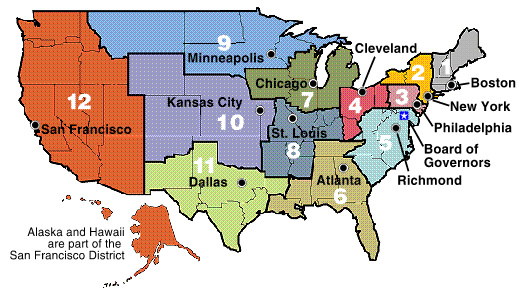
\includegraphics[trim=0 0 0 0,clip,width=0.7\textwidth]{FIGURES/5_Fed}
%	}      %\\
%	%\subfigure{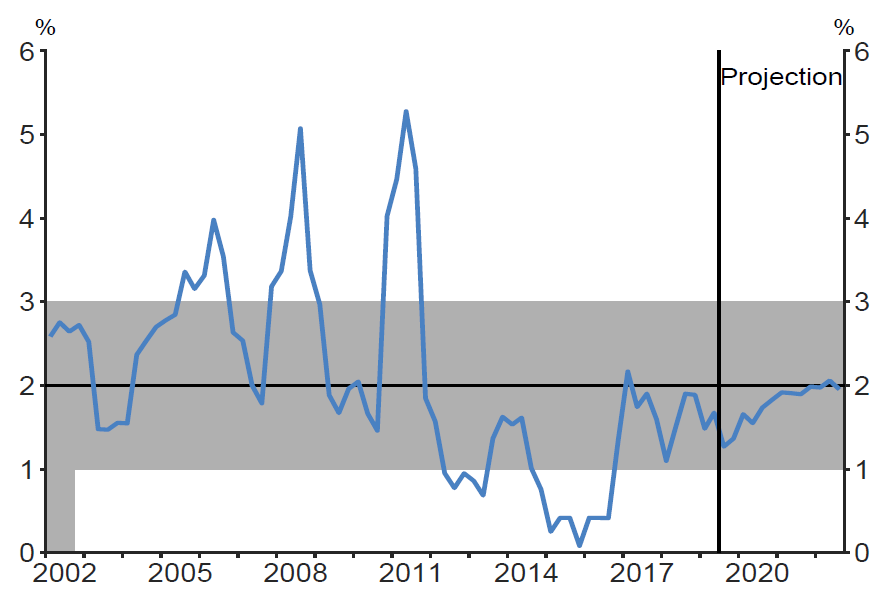
\includegraphics[trim=0 0 0 0,clip,width=0.35\textwidth]{FIGURES/5_NZforecast}
%	%} 
%	
%%	\label{fig:GPD} 
%	%[trim=left bottom right top
%\end{figure}
%%\vspace{-2mm}
%
%%\begin{minipage}{0.9\columnwidth}
%%\tiny	
%%\textbf{Note.} Signatures on US dollar banknote by Rosa Gumataotao Rios and Timothy F. Geithner
%%\textbf{Sources.} Federal Reserve Bank of St. Louis Annual Report 2009, Figure 1. \\
%%\end{minipage}
%\end{center}
%
%\end{frame}
%%---FRAME------------------------------------------------------------------------------
%
%
\end{document}

